\chapter{Implementazione}

%todo intro?


\section{Modifiche hardware alla scheda}\label{s:dw-board-mod}

Come discusso nell'introduzione la scheda \textit{Arduino UNO R3} non presenta alcun supporto al debugging o ad estensioni per tale funzione.

Questo comporta la necessità di sviluppare una nuova scheda derivata dall'architettura di \textit{Arduino UNO} --- il cui sviluppo comporterebbe un dispendio di energie e tempo non indifferenti e alte possibilità di errore --- oppure la modifica hardware e firmware di un esemplare della stessa.

Affinché sia possibile utilizzare l'interfaccia di debugging DebugWire è necessaria una connessione con pull-up diretta con il pin i reset dell'integrato.

Come è possibile osservare dall'allegato~\ref{app:r3-schematic}, L'integrato \texttt{U3} è connesso al pin di reset del target (\texttt{U4}) tramite il condensatore \texttt{C5} (si veda la figura~\ref{fig:r3-schematic-rst-detail}). Sarà dunque necessario rimuovere tale condensatore e ripristinare una connessione diretta tra i micro-controllori come evidenziato dalla figura~\ref{fig:remove-c5}.

\begin{figure}[t]
    \hfill
    \begin{minipage}{.45\textwidth}
        \subfloat[][]{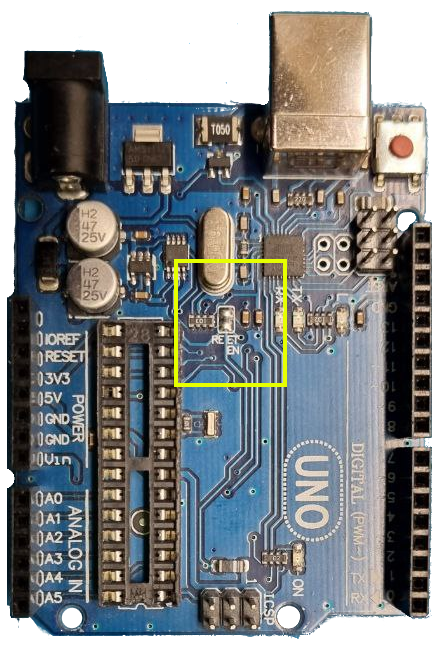
\includegraphics[width=.9\textwidth]{cap_begin.png}}
    \end{minipage}
    \begin{minipage}{.45\textwidth}
        \subfloat[][]{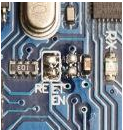
\includegraphics[width=.5\textwidth]{cap_removed.png}} \\
        \subfloat[][]{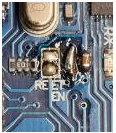
\includegraphics[width=.5\textwidth]{cap_shorted.png}}
    \end{minipage}
    \hfill
    \caption[]{Procedimento di rimozione del condensatore \texttt{C5}. Il condensatore viene rimosso (b) e successivamente la connessione viene ripristinata (c)}\label{fig:remove-c5}
\end{figure}

Tale modifica rende inoperabile il firmware presente sul controllore ATMega16U2 in quanto così facendo la linea di reset rimarrebbe asserita al livello logico 0 durante la durata della connessione con l'\texttt{host}.

Questa modifica comporta però il collegamento i componenti \texttt{RN2D} e \texttt{RN1D} i quali vanno a costituire un partitore di tensione che porrebbe la linea di reset ad un livello logico indefinito ad una tensione di 0.45V. Per questo motivo si rende necessaria una seconda modifica: è necessario isolare la resistenza \texttt{RN2D} tagliando la traccia come mostrato in figura~\ref{fig:cut-rnd2}

\begin{figure}[b]
    \centering
    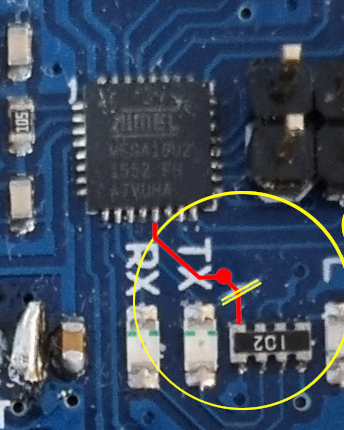
\includegraphics[width=.25\textwidth]{cut_rnd2.png}
    \caption[]{Isolamento del componente \texttt{RN2D} tagliando la traccia evidenziata.}\label{fig:cut-rnd2}
\end{figure}

Questa modifica si ripercuote negativamente sulla possibilità di eseguire il bootloader sull'ATMega16U2, in quanto è necessario che il pin 13 sia posto a 0V perchè esso possa essere caricato. Vi sono quindi tre possibilità:
\begin{enumerate}
    \item Caricare il firmware personalizzato antecedentemente alle modifiche hardware.
    \item Utilizzare un programmatore esterno tramite l'header di programmazione \texttt{ICSP1}
    \item Collegare temporaneamente durante il reset dell'ATMega16U2 la traccia tagliata con l'ausilio di uno strumento conduttivo.
\end{enumerate} 

\subsection{Riutilizzo del pulsante di reset}

La connessione per il debugging, trattasi di una linea seriale open drain, comporta che il punsante di reset presente sulla scheda non sia più funzionante, in quanto le funzionalità originali del pin di reset vengono disattivate con l'attivazione della periferica DebugWire.

La soluzione adottata consiste nell'implementazione di un soft-reset gestito dal microcontrollore ATMega16U2: La connessione del pulsante viene modificata in modo che esso sia un input letto dal firmware modificato del micro-controllore adattatore, il quale si occuperà di resettare il \textit{target} mediante l'invio di una sequenza di comandi descritta dall'algoritmo seguente:
\begin{enumerate}
    \item Halt del target (BREAK)
    \item Reset del controllore (0x07)
    \item Ripresa dell'esecuzione (0x30)
\end{enumerate}

A tal fine è necessario installare una connessione ausiliaria tramite un filo e tagliare la traccia di connessione del pulsante come mostrato dalla figura~\ref{fig:rst-rewire}

\begin{figure}[h]
    \centering
    \subfloat[][]{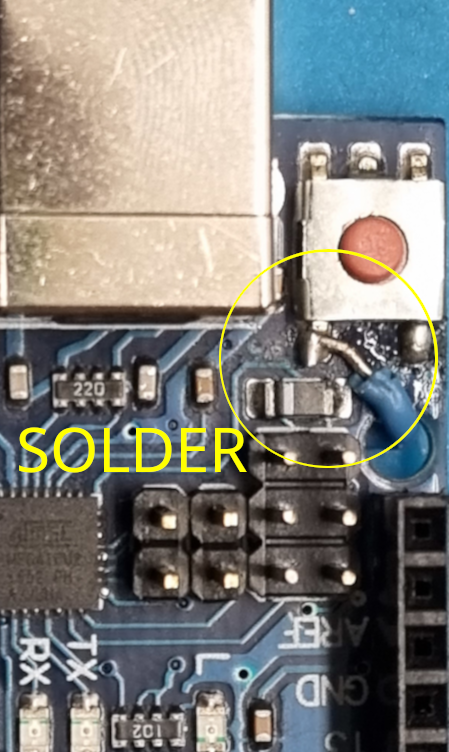
\includegraphics[width=.2\textwidth]{rst-solder-front.png}}
    \hspace{8mm}
    \subfloat[][]{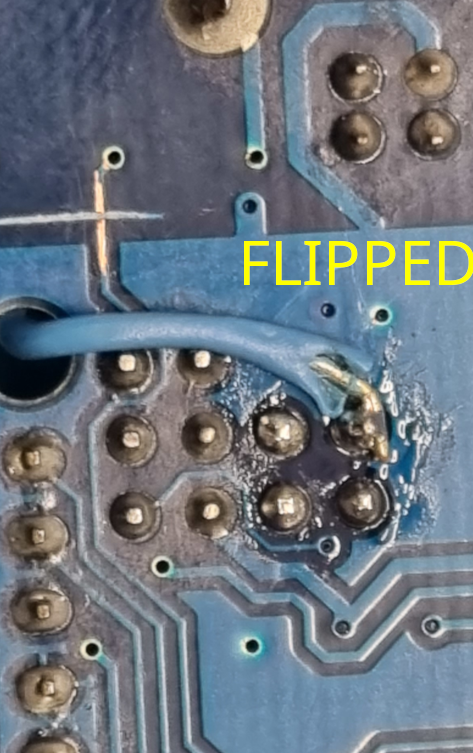
\includegraphics[width=.2\textwidth]{rst-solder-rear.png}}

    \caption[]{Procedimento di isolamento e riutilizzo del pulsante di reset mostrato dal lato superiore (a) e inferiore (b). Si noti la traccia tagliata nell'immagine (b)}\label{fig:rst-rewire}
\end{figure}

\section{Livello Fisico}

Come riportato nella sezione~\ref{ss:dw-phy}, l'interfaccia tra debug server, l'ATMega16U2, e il controllore target è costituita da una linea seriale open drain.

Si rende necessario quindi implementare tale interfaccia in modo efficiente al fine di permettere al server GDB di interfacciarsi con il \textit{target} tramite DebugWire

L'implementazione inizialmente progettata in fase di ideazione, ancora prima che fosse stabilita la piattaforma hardware, sfruttava la periferica UART presente sul controllore ATMega16U2\cite[chap. 18]{avr:m16u2}.

Al fine di implementare l'accesso alla linea open drain si rende necessario l'utilizzo di un componente aggiuntivo come mostrato nella figura~\ref{fig:od-impl}, la quale mostra due alternative di implementazione utilizzando un diodo o un transistor. 

\begin{figure}[t]
    \centering

    \subfloat[][]{
        \begin{circuitikz}
            \draw (0, 0) node[label={[font=\footnotesize]above:rxd}] {} to[short, *-] (2, 0) to[short, -] (2, 1) to[R={\(R_{pullup}\)}] (2, 2) to [short, -] (2, 2.5) to [short, -] (2.5, 2.5) to [short, -] (2.5, 3);
            \draw (2.5, 2.5) to[short, -] (3, 2.5) to[short, -] (3, 2) to[R={\(R1\)}] (3, 1);
            \draw (3,-1) node [npn,xscale=-1,anchor=B] (npn) {\reflectbox{\(Q1\)}} (npn.collector);
            \draw (3, 1) to[short, -] (3, -1);
            \draw (2, 0) to[short, *-*] (4, 0) node[label={[font=\footnotesize]above:target}] {};
            \draw (0, -2) node[label={[font=\footnotesize]above:txd}] {} to[short, *-]  (2.16, -2) to[short, -] (2.16, -1.75);
            \draw (2.16, 0) to[short, *-] (2.16, -0.5);
            \draw (2, 3) -- node[anchor=south,align=center] {VCC} (3, 3);
        \end{circuitikz}
    }
    \subfloat[][]{
        \begin{circuitikz}
            \draw (0, 0) node[label={[font=\footnotesize]above:rxd}] {} to[short, *-] (2, 0) to[short, -] (2, 1) to[R={\(R_{pullup}\)}] (2, 2) to [short, -] (2, 3);
            \draw (1.5, 3) -- node[anchor=south,align=center] {VCC} (2.5, 3);
            \draw (2, 0) to[short, *-*] (4, 0) node[label={[font=\footnotesize]above:target}] {};
            \draw (2, 0) to[short, -] (2, -0.5) to[D={\(D1\)}] (2, -1.5) to[short, -] (2, -2)  to [short, -*] (0, -2) node[label={[font=\footnotesize]above:txd}] {};
        \end{circuitikz}
    }
    \caption[]{L'immagine mostra due possibili circuiti per l'adattamento della periferica UART dell'ATMega16U2 alla linea seriale open drain.}\label{fig:od-impl}
\end{figure}

Il principio di funzionamento dei circuiti in figura~\ref{fig:od-impl} è pressoché identico: Il valore del pin txd viene replicato sulla linea di connessione con un livello logico 0 ``forte'' e un livello logico 0 ``debole'' dato dalla resistenza \(R_{pullup}\) e in entrambi i casi il pin txd viene utilizzato come collettore di corrente.
La differenza consiste nella quantità di componenti aggiuntivi e nelle prestazioni.

Il circuito (a) permette, tramite il pin \textit{txd}, di porre la differenza di potenziale \(V_{be}\) tra base ed emettitore del transistor a circa 5V --- ignorando la caduta di tensione irrilevante sulla resistenza R1 --- permettendo una corrente di base sufficiente a mandare il transistor in saturazione. Questo manda il transistor in conduzione, ed essendo in saturazione, porta la differenza di potenziale \(V_{ce}\) a circa 0.2V imponendo così la tensione sulla connessione verso il target.

Contrariamente il circuito (b) sfrutta il diodo D1 per ottenere lo stesso risultato. La differenza consta nel fatto che nel circuito (a) il transistor permette di avere una caduta di tensione minore essendo in saturazione, cosa che avviene quando il segnale \textit{txd} è zero.

I circuiti sopra mostrati sono verificati dalle simulazioni i cui risultati sono mostrati in figura~\ref{graph:sim}. In aggiunta a quanto esibito, il circuito (b) è stato simulato con un diodo schottky 1N5817 con capacitanza di 125pF per valutarne il comportamento.

\begin{figure}
    \centering
        \begin{tikzpicture}
            \begin{axis}[
                width=0.8\textwidth,
                xlabel={Tempo (S)},
                ylabel={Tensione (V)}
                ]
                \addplot table [x=t, y=v(tgt), col sep=comma, mark=none] {sims/phy-sim-bjt.csv};
                \addplot table [x=t, y=v(txd), col sep=comma, mark=none] {sims/phy-sim-bjt.csv};
                \legend{$tgt$,$txd$}
            \end{axis}
        \end{tikzpicture}\\
        \vfill
        \begin{tikzpicture}
            \begin{axis}[
                width=0.8\textwidth,
                xlabel={Tempo (S)},
                ylabel={Tensione (V)}
                ]
                \addplot table [x=t, y=v(tgt), col sep=comma, mark=none] {sims/phy-sim-diode.csv};
                \addplot table [x=t, y=v(txd), col sep=comma, mark=none] {sims/phy-sim-diode.csv};
                \addplot table [x=Time, y=V(NODE1), col sep=comma, mark=none] {sims/phy-sim-schottky.csv};
                \legend{$tgt (pn)$,$txd$}
            \end{axis}
        \end{tikzpicture}
    \caption[]{Risultati della simulazione dei circuiti in figura~\ref{fig:od-impl} con tempo di bit pari a 8\(\mu\)S}\label{graph:sim}
\end{figure}

Come è possibile notare nel secondo caso la tensione della linea \textit{tgt} non è mai inferiore a 0.7V per la giunzione \textit{pn} mentre nel caso della giunzione metallo-semiconduttore la tensione associata al livello logico 0 è pari a circa 0.15V. Bisogna però sottolineare come nel caso di un diodo schottky l'alta capacitanza causa una lentezza di commutazione non indifferente, essendo che il segnale non raggiunge mai i 5V. 


Sfruttando la periferica UART dell'ATMega16U2 risulta quindi notevolmente semplificata l'implementazione della comunicazione DebugWire, oltre a rendere possibile un approccio ad interrupt per la scrittura del firmware.

\subsection{Implementazione effettiva}

Data la scelta di riutilizzare modificando la scheda \textit{Arduino UNO R3}, si è reso necessario l'utilizzo di un solo pin (pin 13) in quanto già collegato al pin di reset dopo le modifiche apportate descritte dalla sezione~\ref{s:dw-board-mod}.

Di conseguenza si è reso necessario scrivere un'implementazione software del protocollo seriale tramite un solo pin.

La prima difficoltà di impleentazione riguarda la gestione del pin per l'utilizzo OpenDrain: la piattaforma AVR non supporta nativamente in hardware tale funzione, rendendo necessaria la gestione dello stato del pin a livello software.

Vi sono tre registri di gesione di un pin nell'architettura AVR:\ \texttt{PORTx, DDRx e PINx}. A ogni bit di questi registri è associato un pin fisico e il relativo stato.

Attraverso quanto è rappresentato nella figura~\ref{fig:avr-pin} possiamo valutare le varie condizioni nelle quali il pin fisico può trovarsi in funzione dello stato dei bit relativi ai tre registri elencati in precedenza.

\begin{figure}[t]
    \centering
    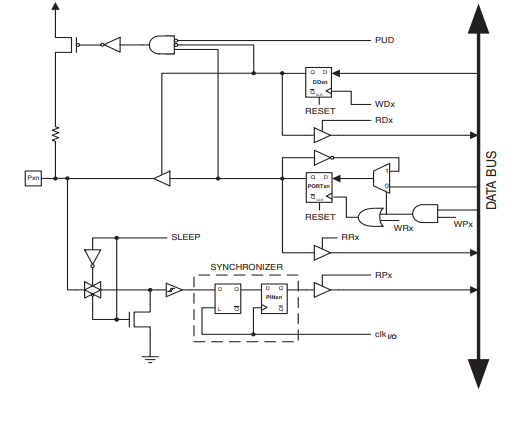
\includegraphics[width=.85\textwidth]{avr-pin-diag.png}
    \caption[Immagine ottenuta dal documento\cite{avr:m16u2}, fig. 12-2]{Diagramma funzionale dell'hardware relativo a un generico pin della famiglia AVR\cite[fig. 12-2]{avr:m16u2}}\label{fig:avr-pin}
\end{figure}

Alla scrittura del registro DDRx viene asserita la linea WDx, la quale salva lo stato del bit associato al pin nel flipflop pilotato da essa. Questo stato pilota un buffer che stabilisce se il pin stesso debba essere un input o un output.

In particolare, se lo stato salvato nel primo flipflop è 1, il pin sarà pilotato con livello logico pari allo stato salvato nel secondo flipflop in modo ``forte''.

Se invece lo stato del pin viene posto come input, ossia lo stato del primo flipflop è 0, è possibile pilotare il FET che alimenta la linea di pullup del pin. Questo accade perchè il segnale che rappresenta la direzione del pin è input negato della porta AND che controlla lo stato del pullup; per questo motivo, lo stato 0 permette alla porta di avere risultato 1 se lo stato del secondo flipflop è pari a 1, in quanto tale segnale sarebbe ignorato perchè il buffer di controllo è disabilitato.

La lettura dello stato del pin può avvenire in qualunque momento tramite la lettura del registro PINx, il quale asserisce la linea RPx e riporta lo stato salvato nello stadio di sincronizzazione.

La scrittura di tale registro viene reindirizzata al controllo del multiplexer in modo da poter invertire lo stato del pin senza averlo precedentemente letto, dimezzando la quantità di operazioni necessarie all'inversione dello stato.

Risulta quindi necessario stabilire due sequenze di operazioni per portare il pin da livello logico basso ``forte'' a livello logico alto ``debole''. In particolare la transizione da livello logico alto a livello logico basso deve avvenire precedentemente alla configurazione della direzione del pin. Questo garantisce che non vi siano possibilità di conflitti potenzialmente catastrofici, considerando il fatto che il segnale che determina l'attivazione del pullup è anche responsabile dello stato del pin. Questo problema risulta evitabile utilizzando un pullup esterno.

Analogamente per la conversione da livello logico basso a livello logico alto il cambio di stato dovrà avvenire successivamente al cambio di direzione.

Così facendo si riducono le possibilità di guasto e si minimizzano i tempi di incertezza --- considerando l'assenza di un pullup esterno --- i quali si limitano al tempo intercorso tra i due cambi di configurazione: ci sarà sempre un intervallo di tempo dove lo stato del pin sarà posto a livello logico basso e il pin posto in configurazione di input, lasciando così la connessione flottante.

In questi casi, data la durata di natura molto breve della commutazione e del periodo di incertezza, la capacitanza parassita della connessione permetterà di mantenere un livello logico costante.

\subsubsection{Implementazione del protocollo di comunicazione}

L'implementazione della comunicazione seriale emulata a livello software è soggetta a vincoli relativi al tempo di esecuzione.

L'implementazione si basa sull'utilizzo del timer TIMER1, un timer a 16 bit in grado di generare interrupt di comparazione e sul rilevamento della caduta da livello logico alto a basso per identificare un bit di inizio trasmissione.

Il concetto sul quale si basa il funzionamento consiste nel mantenere il timer in esecuzione ed eventualmente resettarne il conteggio nel caso si renda necessario una re-sincronizzazione in ricezione.

Entrambe le azioni di trasmissione e ricezione vengono implementate come una macchina a stati la quale iterazione è controllata dall'interrupt di comparazione di TIMER1.

Entrambe le funzionalità sono divide in due domini di esecuzione: l'esecuzione invocata dall'utente e la macchina a stati relativa eseguita con l'interrupt. 

La funzionalità di invio è implementata tramite un meccanismo di accodamento per due processi producer/consumer: alla prima invocazione della funzione di invio il byte viene salvato nella coda e viene abilitata la macchina a stati mostrata in figura~\ref{fig:phy-state-tx} tramite il flag \texttt{\_OD\_UART\_BUSY} la quale consumerà il dato al primo interrupt di comparazione, mentre nella seconda invocazione un secondo byte verrà inserito nella coda e la funzione potrà ritornare liberamente. 

È compito della macchina a stati riconoscere che un secondo byte è stato aggiunto alla coda \texttt{OD\_UART\_TX\_FULL} e di conseguenza essa inizierà una nuova trasmissione invece che andare allo stato \texttt{IDLE}.

\begin{figure}[t]
    \centering
    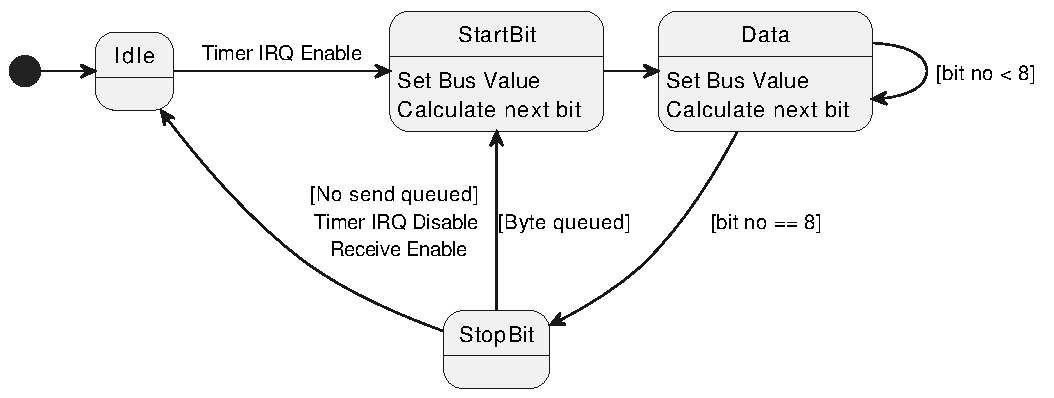
\includegraphics[width=.95\textwidth]{phy-tx-state.pdf}
    \caption[]{Macchina a stati per l'implementazione della trasmissione seriale}\label{fig:phy-state-tx}
\end{figure}

Il comportamento sopra descritto viene riassunto dalla figura~\ref{fig:phy-tx-timing}. Si noti come i cambiamenti di stato e il calcolo dei valori avvenga nell'iterazione precedente all'attuazione.
Inoltre l'immagine mostra come un eventuale aggiunta di un dato alla coda persista e venga indicata dal flag \texttt{OD\_UART\_TX\_FULL}.

Una volta terminata l'esecuzione dell'invio del dato, essendoci un ulteriore byte in coda, viene ripresa l'esecuzione immediatamente.

\begin{figure}[p]
    \checkoddpage%
    \ifoddpage%
        \begin{adjustbox}{addcode={\begin{minipage}{\width}}{\caption[]{%
            Diagramma delle tempistiche di esecuzione dell'invio di dati sulla linea seriale implementata via software.}\label{fig:phy-tx-timing}\end{minipage}},rotate=90,center}
            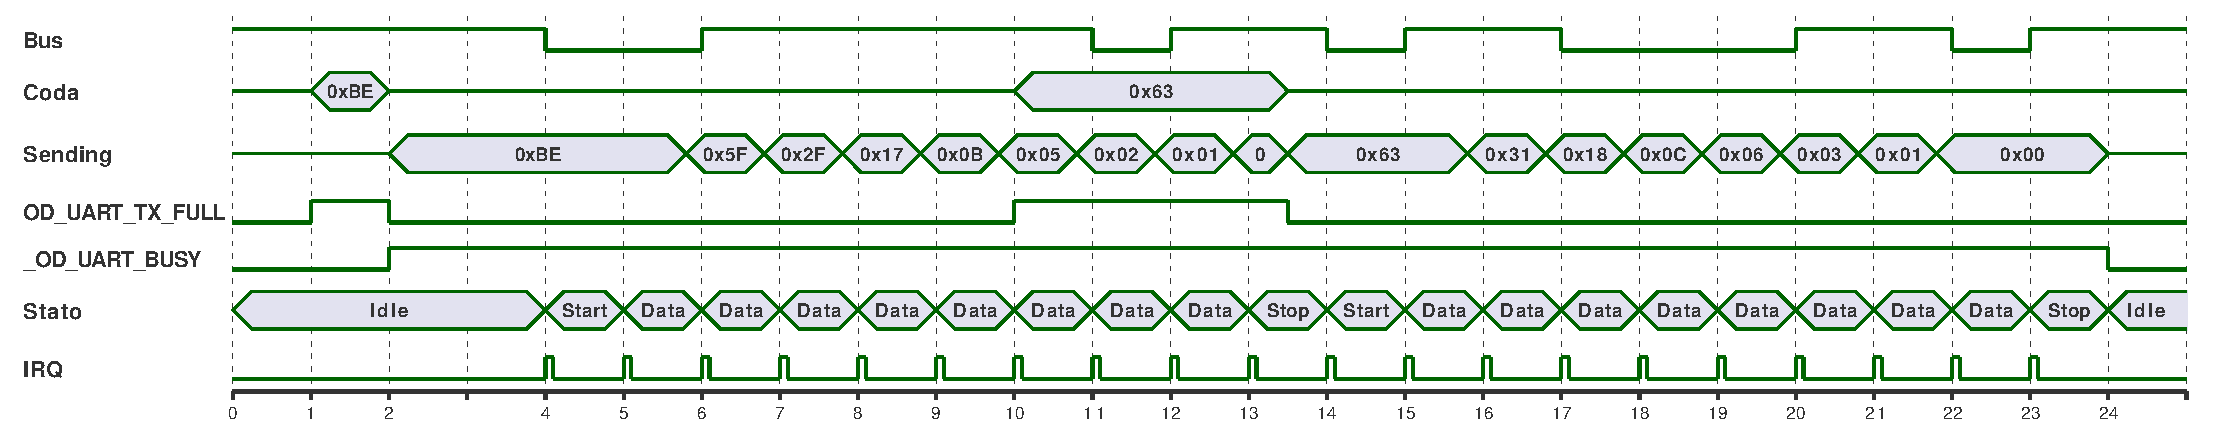
\includegraphics[width=\textheight]{phy-tx-timing.pdf}%
        \end{adjustbox}
    \else
        \begin{adjustbox}{addcode={\begin{minipage}{\width}}{\caption[]{%
            Diagramma delle tempistiche di esecuzione dell'invio di dati sulla linea seriale implementata via software.}\label{fig:phy-tx-timing}\end{minipage}},rotate=-90,center}
            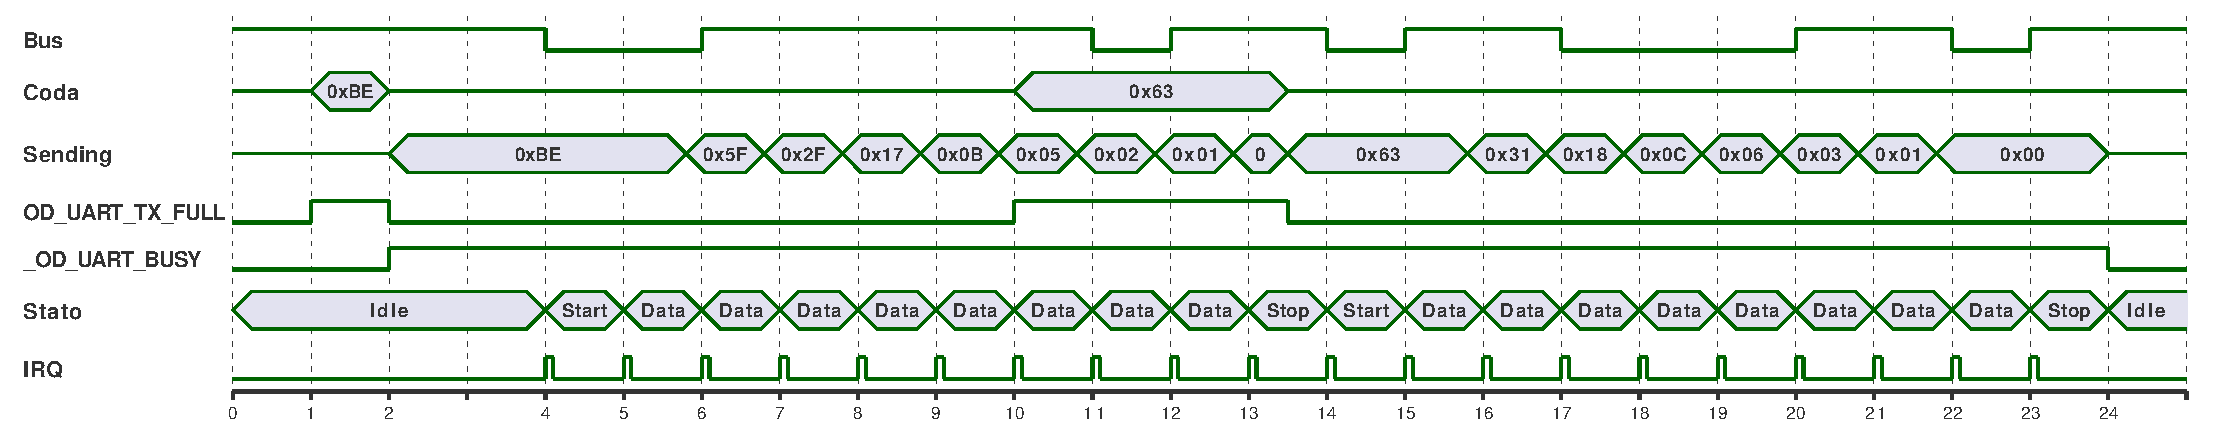
\includegraphics[width=\textheight]{phy-tx-timing.pdf}%
        \end{adjustbox}
    \fi
\end{figure}



La parte di ricezione viene implementata con una seconda macchina a stati mostrata in figura~\ref{fig:phy-rx-state} ma il primo passaggio di stato, da Idle a StartBit avviene alla ricezione di un interrupt relativo al cambiamento di stato del bus.

La ragione per cui questo passaggio debba avvenire all'avvenimento di un interrupt consiste nel fatto che il \textit{target} può inviare una risposta in qualsiasi istante temporale.

Risulta quindi necessario l'utilizzo di una struttura FIFO per il salvataggio dei dati ricevuti dalla quale poi l'utente potrà attingere durante l'esecuzione del software. In particolare il flag \texttt{\_OD\_UART\_AVAIL} indicherà la presenza di dati non ancora letti nel buffer.

Si rende quindi necessario poter ripristinare il conteggio del TIMER1 al fine di re-sincronizzare il clock di campionamento del bus al centro del bit per i motivi descritti nella sezione~\ref{ss:uart}, in particolare facendo riferimento all'equazione~\ref{eq:uart-period-receive-delay}. Questo comportamento è riassunto dalla figura~\ref{fig:phy-rx-timing}.

Alla ricezione dell'interrupt di cambio di stato la macchina a stati viene inizializzata e il timer resettato in modo che il successivo interrupt di comparazione avvenga a metà del bit successivo. Ad ogni interrupt il valore del bus viene aggiunto secondo l'equazione~\ref{eq:rx-push} al valore temporaneo fino al raggiungimento delle otto iterazioni. A questo punto lo stato passa a \texttt{StopBit}, dove il valore temporaneo viene inserito nella coda e viene asserito il flag \texttt{\_OD\_UART\_AVAIL}.

\begin{equation}\label{eq:rx-push}
    tmp_{i+1} = (bus << 7) | (tmp_i >> 1)
\end{equation}

\begin{figure}[p]
    \centering
    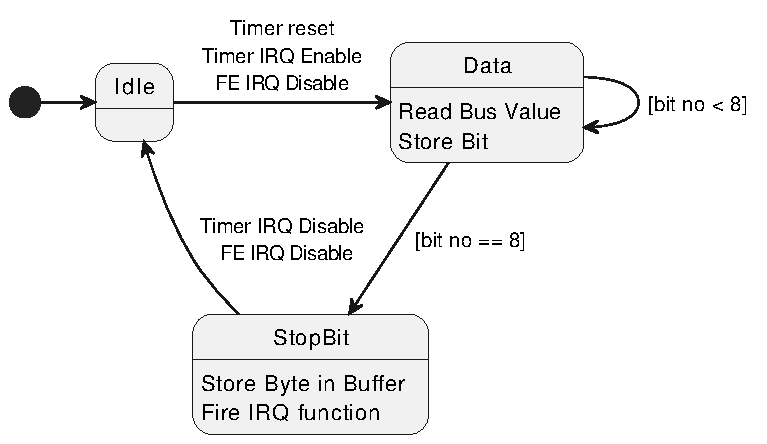
\includegraphics[width=.75\textwidth]{phy-rx-state.pdf}
    \caption[]{Macchina a stati relativa alla ricezione della seriale implementata in software.}\label{fig:phy-rx-state}
\end{figure}

\begin{figure}[p]
    \centering
    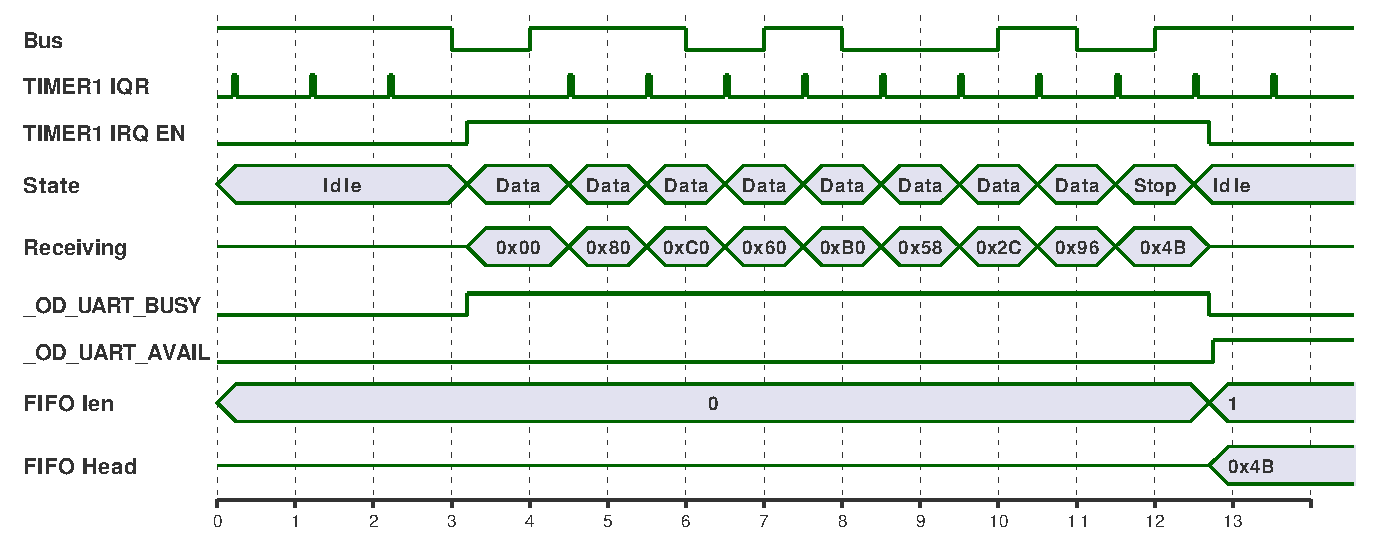
\includegraphics[width=.99\textwidth]{phy-rx-timing.pdf}
    \caption[]{Macchina a stati relativa alla ricezione della seriale implementata in software.}\label{fig:phy-rx-timing}
\end{figure}

Il listato~\ref{lst:fe-irq-management} mostra il frammento di codice per la gestione dell'inizio ricezione. 

\noindent\begin{minipage}{\textwidth}
    \begin{lstlisting}[style=C, caption={IRQ di gestione inizio trasmissione}, label=lst:fe-irq-management]
__attribute__((optimize("-Ofast"))) ISR(INT7_vect){
    cli();
    FE_IRQ_DISABLE(); //start a new rx. clear irq
    fast_flags = 0;
    uart_flags |= OD_UART_FLAG_BUSY_MASK; //set busy flag, reset flags
    TCNT1 = 0; //set counter to start at next bit. make correction for timer startup and bad things.
    TIMER_IRQ_ENABLE(); //enable timer and clear irq
    TIMER_IRQ_CLEAR();
    sei();
}
    \end{lstlisting}
\end{minipage}

È possibile osservare come nella compilazione dell'handler dell'interrupt venga privilegiata la velocità di esecuzione anziché lo spazio occupato dal compilato, e come il TIMER1 venga impostato a 0. Così facendo il campionamento avverrà verso l'inizio del bit inviato anziché alla metà del tempo di bit. 

Questo non è da considerarsi un problema data la bassa frequenza dell'insieme.

È inoltre necessario impostare \texttt{TCNT1 = OCR1A >\textcompwordmark> 2} nel caso si voglia utilizzare frequenze vicine a 125000 bit per secondo in quanto vanno considerati i tempi di esecuzione del codice e di reazione del timer. Questo valore è stato trovato sperimentalmente mediante l'uso di un analizzatore logico.

\section{DebugWire}

Grazie alla possibilità di eseguire istruzioni arbitrarie tramite l'interfaccia di debug, è possibile creare delle funzionalità non previste dal protocollo stesso ma di notevole importanza per la gestione del debug.

\subsection{Riconoscimento del target}

Durante l'inizializzazione il debugger leggerà il registro SIGNATURE DebugWire per identificare il componente.

Una sezione di memoria flash è stata dedicata al salvataggio di una struttura dati contenente le informazioni necessarie al debugging di un integrato, per cui è sufficiente cercare sequenzialmente la coincidenza del valore del registro signature rispetto al campo id.

La struttura salvata contenente gli indirizzi e le dimensioni viene mostrata con il listato~\ref{lst:struct-dw-dev}

\noindent\begin{minipage}{\textwidth}
    \begin{lstlisting}[style=C, caption={Strutture utilizzate nel codice finale per il salvataggio e la ricerca dei parametri associati al target connesso}, label=lst:struct-dw-dev]
    typedef struct dw_device_definition{
        uint16_t signature;

        uint16_t sram_base;         //first sram address after extended io
        uint16_t sram_end;          //first sram address after extended io

        uint8_t flash_page_end;     //words per page
        uint16_t flash_end;         //last flash valid word

        uint16_t eeprom_end;        //first eeporom address after io and extended io

        uint8_t reg_spmcsr;
        uint8_t reg_dwdr;
        uint8_t reg_eearl;
        uint8_t reg_eecr;
        uint8_t reg_eedr;
    } __attribute__((packed)) dw_device_definition_t;

    struct dw_devices{
        uint16_t items;
        dw_device_definition_t devices[];
    } __attribute__((packed));
    \end{lstlisting}
\end{minipage}

\subsection{Programmazione delle memorie non volatili}

In particolare il protocollo DebugWire non permette di accedere in scrittura alle memorie non volatili, impedendone così la programmazione tramite tale interfaccia.

Prendendo spunto da quanto riportato sul datasheet della maggior parte dei dispositivi AVR\cite[34]{avr:m328p}\cite[sec 26.2.5]{avr:m328p}, è possibile ideare una breve routine eseguibile passo-passo dal debugger per la scrittura di tali memorie.

Bisogna però trovare un modo per inviare il dato, o i dati, da scrivere nella memoria.

Una possibile soluzione potrebbe essere quella di scrivere il byte o la pagina in RAM e utilizzare così istruzioni \texttt{ld}, ma questo approccio richiederebbe troppe istruzioni e causerebbe lunghi tempi di programmazione.

La soluzione adottata è quella di leggere o scrivere il registro \texttt{DWDR}. Dati i test eseguiti, una scrittura del registro tramite i comandi sopra descritti (il registro si trova ad un indirizzo noto) richiede un ulteriore byte inviato sulla linea seriale che verrà salvato in tale registro\cite{site:dw-reverse-engeneering}. Analogamente la sua lettura comporta un ulteriore byte inviato dal target rappresentate il valore salvato\cite{site:dw-reverse-engeneering}.

Sono stati elaborati due frammenti di codice eseguibili dal debugger per la programmazione delle memorie non volati. Essi sono consultabili nell'appendice come documento~\ref{app:dw-flash-prog} e documento~\ref{app:dw-eeprom-prog}.

Da tali documenti possiamo osservare come il codice sia fortemente dipendente dal debugger per la preparazione del contesto, ovvero necessita che prima dell'esecuzione siano eseguite certe istruzioni di preparazione quali salvataggio dello stato dei registri e preparazione delle costanti e indirizzi nei registri utilizzati.

Inoltre la scrittura dell'algoritmo di programmazione della memoria flash è stata fatta facendo sì che non sia necessario istanziare un buffer contenente l'intera pagina da programmare precedentemente alla chiamata, bensì è possibile scrivere il buffer temporaneo a blocchi di dimensione indefinita purché venga completato prima di procedere.

Questo permette di scrivere codice a bassissimo impatto sulla quantità di memoria SRAM utilizzata per buffer temporanei, condizione necessaria per lo sviluppo su ATMega16U2 in quanto la memoria SRAM totale disponibile non supera i 512byte\cite{avr:m16u2}.

\subsection{Salvataggio stato di esecuzione}

Come anticipato in precedenza, l'esecuzione di azioni tramite debug wire comporta la sovrascrittura di alcuni registri al fine di configurare le azioni prima dell'operando GO, come mostrato dalle figure~\ref{fig:dw-reg-rw-com}~e~\ref{fig:dw-mem-rw-com}, comportando così una modifica dello stato dei registri inattesa e imprevedibile dal firmware in esecuzione.

Il solo cambio del valore del Program Counter comporterebbe la ripresa dell'esecuzione da un punto arbitrario del codice compilato senza alcun contesto logico.

È quindi necessario creare un sistema di salvataggio temporaneo dello stato in SRAM permettendone così il ripristino al termine delle operazioni.

A tal fine è stata identificata l'interdipendenza delle operazioni DebugWire e il loro utilizzo dei registri come mostrato dalla figura~\ref{fig:dw-wrt-deps}

\begin{figure}[h]
    \centering

    \resizebox{.95\textwidth}{!}{%
        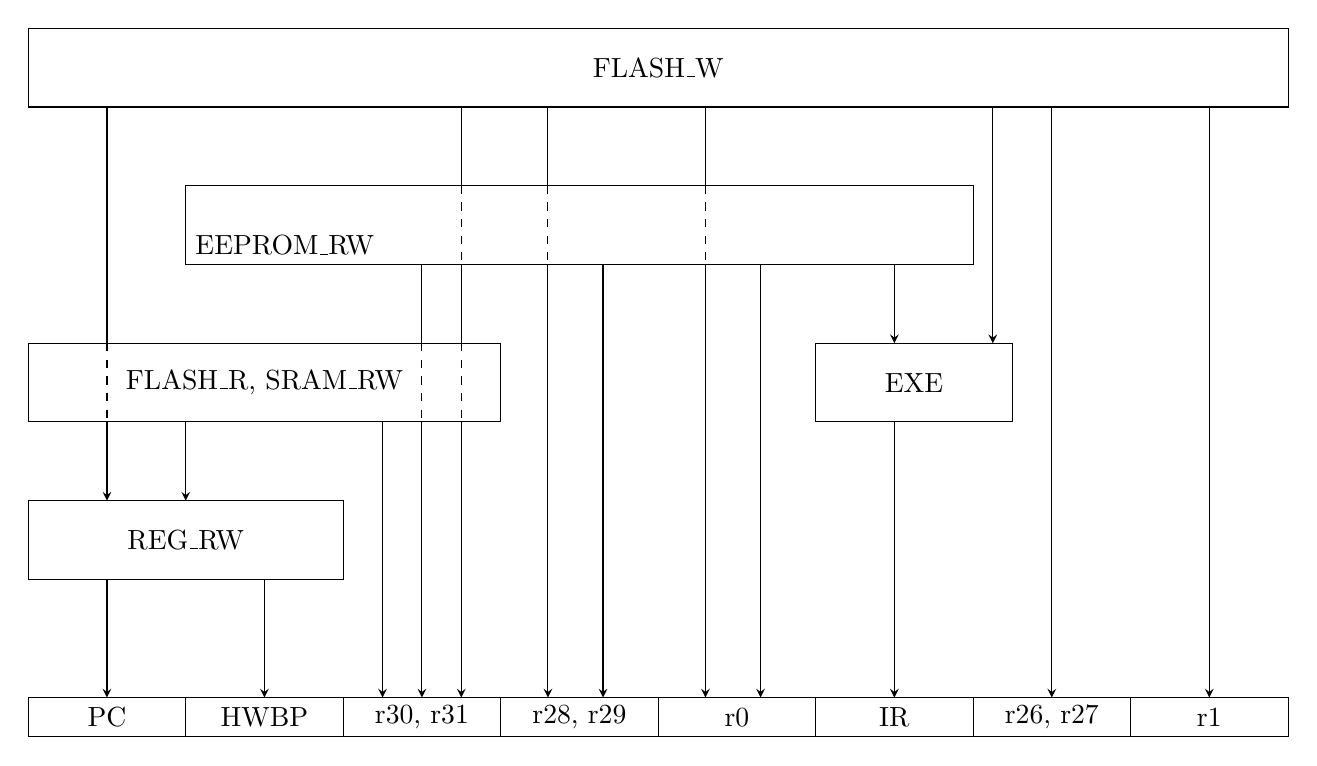
\begin{tikzpicture}
            \draw (0,0) rectangle (2, 0.5) node[pos=.5] {PC};
            \draw (2,0) rectangle (4, 0.5) node[pos=.5] {HWBP};
            \draw (4,0) rectangle (6, 0.5) node[pos=.5] {r30, r31};
            \draw (6,0) rectangle (8, 0.5) node[pos=.5] {r28, r29};
            \draw (8,0) rectangle (10, 0.5) node[pos=.5] {r0};
            \draw (10,0) rectangle (12, 0.5) node[pos=.5] {IR};
            \draw (12,0) rectangle (14, 0.5) node[pos=.5] {r26, r27};
            \draw (14,0) rectangle (16, 0.5) node[pos=.5] {r1};
            \draw (0, 2) rectangle (4, 3) node[pos=.5] {REG\_RW};
            \draw (0, 4) rectangle (6, 5) node[pos=.5] {FLASH\_R, SRAM\_RW};
            \draw (10, 4) rectangle (12.5, 5) node[pos=.5] {EXE};
            \draw (12, 7) rectangle (2, 6) node[anchor=south west] {EEPROM\_RW};
            \draw (0, 8) rectangle (16, 9) node[pos=.5] {FLASH\_W};

            \draw [-stealth](1, 2) -- (1, 0.5);
            \draw [-stealth](3, 2) -- (3, 0.5);
            \draw [-stealth](4.5, 4) -- (4.5, 0.5);
            \draw [-stealth](7.3, 6) -- (7.3, 0.5);
            \draw [-stealth](9.3, 6) -- (9.3, 0.5);
            \draw [-stealth](11, 4) -- (11, 0.5);
            \draw [-stealth](13, 8) -- (13, 0.5);
            \draw [-stealth](15, 8) -- (15, 0.5);

            \draw [-stealth](2, 4) -- (2, 3);
            \draw [-stealth](11, 6) -- (11, 5);
            \draw [-stealth](12.25, 8) -- (12.25, 5);

            \draw (6.6, 8) -- (6.6, 7);
            \draw [dashed](6.6, 7) -- (6.6, 6);
            \draw [-stealth](6.6, 6) -- (6.6, 0.5);

            \draw (8.6, 8) -- (8.6, 7);
            \draw [dashed](8.6, 7) -- (8.6, 6);
            \draw [-stealth](8.6, 6) -- (8.6, 0.5);

            \draw (1, 8) -- (1, 5);
            \draw [dashed](1, 5) -- (1, 4);
            \draw [-stealth](1, 4) -- (1, 3);

            \draw (5, 6) -- (5, 5);
            \draw [dashed](5, 5) -- (5, 4);
            \draw [-stealth](5, 4) -- (5, 0.5);

            \draw (5.5, 8) -- (5.5, 7);
            \draw [dashed](5.5, 7) -- (5.5, 6);
            \draw (5.5, 6) -- (5.5, 5);
            \draw [dashed](5.5, 5) -- (5.5, 4);
            \draw [-stealth](5.5, 4) -- (5.5, 0.5);
        \end{tikzpicture}
    }

    \caption[]{Diagramma delle dipendenze di utilizzo dei registri target per le azioni DebugWire}\label{fig:dw-wrt-deps}
\end{figure}

È possibile individuare un cammino comune di salvataggio e ripristino dei registri per tutte le operazioni. In particolare è evidente come tutte le operazioni, ad eccezione di \texttt{EXE}, dipendano da \texttt{REG\_RW}, e come le operazioni di scrittura sulle memorie non volatili dipendano da scritture sugli stessi registri di \texttt{SRAM\_RW}.

La sequenza di salvataggio e ripristino viene mostrata nella la figura~\ref{fig:dw-wrt-seq}. L'immagine mostra una pila di registri per la quale, dato un punto di ingresso comune in funzione dell'azione da eseguire, sarà necessario salvare tutti i registri visitati nella discesa della pila fino al punto di uscita definito da tale operazione. Per esempio, l'azione \texttt{EEPROM\_RW} dovrà salvare i registri \texttt{PC}, \texttt{HWBP}, \texttt{Z (r30, r31)}, \texttt{IR}, \texttt{Y(r26, r27)} e \texttt{r0}. È possibile notare come i registri elencati siano anche quelli utilizzati dal codice presente al documento in appendice~\ref{app:dw-eeprom-prog}

\begin{figure}[h]
    \centering
    %\resizebox{.95\textwidth}{!}{%
        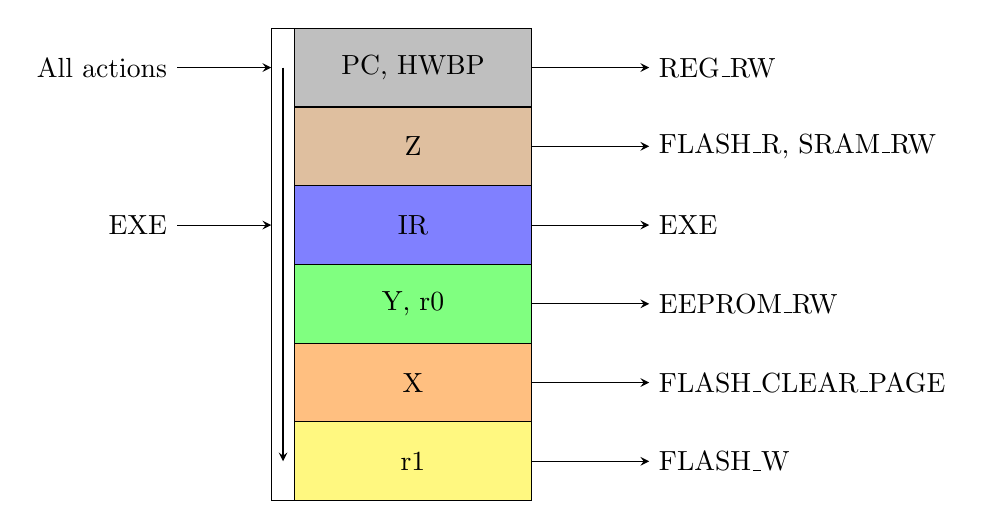
\begin{tikzpicture}
            
            \draw [fill=yellow!50] (0,0) rectangle (3, 1) node[pos=.5] {r1};
            \draw [fill=orange!50] (0,1) rectangle (3, 2) node[pos=.5] {X};
            \draw [fill=green!50] (0,2) rectangle (3, 3) node[pos=.5] {Y, r0};
            \draw [fill=blue!50] (0,3) rectangle (3, 4) node[pos=.5] {IR};
            \draw [fill=brown!50] (0,4) rectangle (3, 5) node[pos=.5] {Z};
            \draw [fill=gray!50] (0,5) rectangle (3, 6) node[pos=.5] {PC, HWBP};

            \draw (-0.3, 0) rectangle (0, 6);
            \draw [-stealth] (-0.15, 5.5) -- (-0.15, 0.5);

            \draw [stealth-] (-0.3, 5.5) -- (-1.5, 5.5) node[left] {All actions};
            \draw [stealth-] (-0.3, 3.5) -- (-1.5, 3.5) node[left] {EXE};

            \draw [-stealth] (3, 5.5) -- (4.5, 5.5) node[right] {REG\_RW};
            \draw [-stealth] (3, 4.5) -- (4.5, 4.5) node[right] {FLASH\_R, SRAM\_RW};
            \draw [-stealth] (3, 2.5) -- (4.5, 2.5) node[right] {EEPROM\_RW};
            \draw [-stealth] (3, 1.5) -- (4.5, 1.5) node[right] {FLASH\_CLEAR\_PAGE};
            \draw [-stealth] (3, 0.5) -- (4.5, 0.5) node[right] {FLASH\_W};
            \draw [-stealth] (3, 3.5) -- (4.5, 3.5) node[right] {EXE};
        \end{tikzpicture}
    %}

    \caption[]{Diagramma dei salvataggi e ripristini dei registri in funzione dell'operazione da eseguire}\label{fig:dw-wrt-seq}
\end{figure}

\subsection{Software Breakpoints}

L'aggiunta della possibilità di scrivere la memoria flash consente l'implementazione dei software breakpoints.

Un breakpoint è un indicatore associato a un indirizzo di memoria dove il codice è in esecuzione con il fine di interrompere l'esecuzione dell'algoritmo e passare il controllo al debugger per effettuare le operazioni di analisi e ispezione.

Questi consistono nella sovrascrittura di un'istruzione con l'opcode corrispondente a \texttt{BREAK} causando così l'halt della cpu e l'intervento del debugger prima dell'esecuzione della stessa.
Alla ripresa dell'esecuzione il debugger caricherà in memoria l'istruzione originale e riprenderà il flusso del codice.

Un primo approccio per la scrittura del codice relativo a questa feature consiste nell'aggiornare la memoria flash scrivendo un'istruzione BREAK\footnote{0x0000} non appena possibile e salvare in una struttura dati la coppia \[<indirizzo>:<opcode>\]

Un possibile algoritmo viene esibito di seguito. Questo algoritmo ha un impatto sull'utilizzo della memoria SRAM di 18 byte facendo uso del fatto che è possibile riempire il buffer di scrittura prima della cancellazione della pagina.

Sia \(address\) l'indirizzo dell'istruzione da sostituire (word address), \(pagelen\) il numero di word in una pagina.

\begin{enumerate}
    \item Salvataggio dei registri come definito in figura~\ref{fig:dw-wrt-seq} per l'azione \texttt{FLASH\_W} (14 byte)
    \item Poniamo l'indirizzo di pagina, utilizzando 2 byte, come \[pageaddr = \left\lfloor\frac{address}{pagelen}\right\rfloor pagelen\] 
    \item Iniziamo la scrittura di una pagina e, per ogni indirizzo da \(pageaddr\) a \(address\) (escluso), leggiamo in una variabile temporanea (2 byte) il valore della memoria flash a quell'indirizzo e aggiungiamo al buffer di scrittura presente nell'integrato.
    \item Scriviamo del buffer l'istruzione BREAK.\@ 
    \item Per ogni indirizzo da \(address + 1\) a \(pageaddr + pagelen - 1\) popoliamo il buffer con quanto letto. 
    \item Eseguiamo l'azione Page Clear all'indirizzo \(pageaddr\)
    \item Eseguiamo l'azione di programmazione della pagina.
    \item Ripristiniamo lo stato dei registri invertendo quanto eseguito al punto 1.
\end{enumerate}

Quanto riportato, seppur una soluzione valida, causa un deterioramento della memoria flash e innalza notevolmente i tempi di debug, inserendo attese notevoli tra il posizionamento di un breakpoint e un altro.

L'algoritmo finale risolve queste problematiche adottando una gestione ``\textit{lazy}'' dei breakpoint e accorpando modifiche alle pagine di memoria flash solo al momento precedente all'esecuzione.
Questo permette di evitare tutte le riscritture date dall'eventuale indecisione del programmatore o errori di puntamento.

Un breakpoint software viene definito con la struttura presentata nel listato~\ref{lst:dw-swbp-struct}. I flag \texttt{active} e \texttt{stored} permettono di identificare le azioni da intraprendere al momento dell'applicazione delle modifiche in memoria.

\noindent\begin{minipage}{\textwidth}
    \begin{lstlisting}[style=C, caption={Struttura utilizzata per il salvataggio dei riferimenti ai breakpoint software}, label=lst:dw-swbp-struct]
    typedef struct dw_sw_brkpt{
        uint16_t address;
        uint16_t opcode;

        uint8_t active : 1;
        uint8_t stored : 1;
    } dw_sw_brkpt_t;
    \end{lstlisting}
\end{minipage}

In particolare si ha che è necessario eseguire un'azione in memoria se i due flag sono discordanti: se un breakpoint è stato abilitato ma non è stato scritto in memoria sarà necessario sostituire l'istruzione presente all'indirizzo \(address\), mentre se un breakpoint è salvato (\texttt{stored} = 1) ma disabilitato sarà necessario ripristinare \(opcode\) all'indirizzo specificato.

Nel caso di aggiunta o rimozione di un breakpoint l'indirizzo viene ricercato all'interno della lista di breakpoint precedentemente definiti comparando l'indirizzo. Se il breakpoint era stato precedentemente definito allora il riferimento viene modificato impostando la variabile \texttt{active} al valore consono. In caso contrario viene creato un nuovo riferimento in coda.

Prima della ripresa dell'esecuzione la lista di breakpoint viene ordinata mediante insertion sort secondo in seguenti criteri:
\begin{itemize}
    \item se due riferimenti sono entrambi non salvati e inattivi non viene effettuata l'inversione e sono considerati uguali ignorando l'indirizzo.
    \item se il primo riferimento è inattivo e non salvato mentre il secondo è o salvato o attivato, allora viene eseguita l'inversione
    \item se sono tutti e due attivi o salvati, vengono comparati gli indirizzi e avviene l'inversione se il primo indirizzo è maggiore del secondo.
\end{itemize}

Così facendo si ottiene una lista di riferimenti ordinati per indirizzo crescente con i riferimenti da eliminare posti in coda a scapito di quest'ultimo, permettendo quindi la rimozione dei riferimenti inattivi e non salvati perché non più esistenti partendo dal fondo e eliminando fino a trovare un riferimento attivo o salvato.

Ora risulta possibile accorpare le scritture in memoria con un algoritmo simile a quanto riportato in precedenza considerando però la presenza di più breakpoint per pagina.

Sarebbe possibile rendere la ricerca e l'ordinamento più efficiente utilizzando algoritmi quali ricerca binaria e qsort ma non è stati ritenuto necessario essendo il numero massimo di riferimenti limitato a venti.

\section{Server GDB}

\section{Real Time Terminal}

Come precedentemente anticipato, questo progetto mira a costituire un insieme di strumenti e funzionalità per il supporto del programmatore alla programmazione nel mondo embedded AVR.\@

Nei capitoli precedenti è stata discussa l'implementazione di un server GDB per effettuare il debugging sul controllore e permettere l'ispezione in loco degli effetti dei programmi e l'alterazione delle risorse durante l'esecuzione a fini diagnostici. 

Affiancata alla pratica del debugging possiamo classificare un'altro metodo diagnostico: il \textit{logging}.

Questa seconda pratica --- spesso usata in modo scorretto per analizzare un problema in una porzione di codice --- consente di generare messaggi analizzabili successivamente a fine di \textit{auditing}, ovvero l'analisi di messaggi di log passati per individuare malfunzionamenti o vulnerabilità inattesi e imprevisti.

I messaggi di log sono anche utili per individuare in quale macro area del codice si trova un possibile baco per poi indagare tramite debugger una volta identificata la causa scatenante.

La questione diviene velocemente come implementare tale funzionalità sulla piattaforma AVR.\@ La maggior parte dei progetti e delle piattaforme utilizza la periferica UART del target al fine di comunicare con l'host impedendone così l'utilizzo da parte del programmatore per comunicare con altre periferiche. Alcune piattaforme hanno ottimizzato questo utilizzo dedicando la linea seriale anche alla programmazione, riducendo però lo spazio disponibile nella memoria flash in quanto tale operazione deve essere svolta da un programmatore. 